\chapter{Polarization of a transverse electromagnetic wave (2)}\label{lec:lec24}
Polarization can be defined as the behaviour or variation of an electric wave as a function of time at a given point in space. Polarization can be categorized into three; 
\begin{enumerate}[(i)]
\item Linear polarization
\item Circular polarization
\item Elliptical polarization
\end{enumerate}
The linear and circular are special cases of the elliptical polarization and also the circular and elliptical polarization possesses a sense of direction. The state of polarization can be defined using certain parameters.
\begin{enumerate}[(i)]
\item Wave parameters $(\epsilon,\tau)$
\newline where: $\epsilon$ = $\cot^{-1}(AR)$
\item Electrical parameters $(\gamma, \delta)$
\newline	where: $\gamma$ = $\tan^{-1} (\frac{E_{2}}{E_{1}})$
\end{enumerate}
Two pairs of angles have been used to describe the state of polarization in both cases to have a compact representation as ($\epsilon$, $\tau$)  or ($\gamma$, $\delta$).

\section{Poincare sphere}
A compact representation of all possible states of polarization with points marked out in a sphere is represented by what is called a POINCARE SPHERE\footnote{The method of the Poincare sphere was proposed by Henri Poincare, a French mathematician, theoretical physicist, engineer and philosopher of science in 1891-1892. It is a convenient approach to represent polarized light.}\index{poincare sphere}.

Taking a look at the state of polarization, we have an axial ratio ranging from 1 to $\infty$, the tilt angle $\tau$ varies from 0 to $180^{o}$, phase difference $\delta$ varies from $-90^{o} to +90^{o}$.

So now we have the range for all these parameters. With Axial ratio AR ranging from 1 to $\infty$, 

$\cot^{-1}(1)= \dfrac{\pi}{4}$

$\cot^{-1}(\infty)= 0$.

$\cot^{-1}(-1) = -\dfrac{\pi}{4}$, 

$\cot^{-1}(-\infty) = 0$

So we have,  0 $\leq$ $\gamma$ $\leq$ $\pi$  and $\dfrac{-\pi}{2}$ $\leq$ $\delta$ $\leq$ $\dfrac{\pi}{2}$ for electrical parameters.

For ellipse(wave) parameters, $\dfrac{-\pi}{4}$ $\leq$ $\epsilon$ $\leq$ $\dfrac{\pi}{4}$ and 0 $\leq$ $\tau$ $\leq$ $\pi$.

So states of polarization are defined by a pair of angles ($\gamma$, $\delta$) or ($\epsilon$, $\tau$). Once these angles were defined, a nice way was found to represent the angles in a compact form. It was realized that a sphere can be constructed such that, every point on the sphere can be uniquely represented by either ($\gamma$, $\delta$) or ($\epsilon$, $\tau$). Once we have this compact representation essentially, we have a sort of visual representation of the state of polarization. 

Let us imagine a sphere with the angles on the sphere marked in terms of either ($\gamma$, $\delta$) or ($\epsilon$, $\tau$). We will have a sphere with latitude and longitude lines drawn on it as shown below.
\begin{figure}[h]
\centering
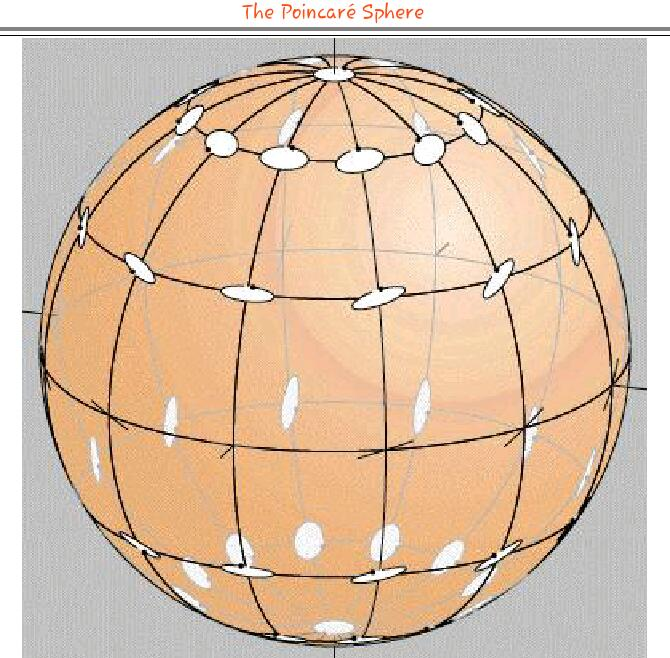
\includegraphics[height=5cm]{./graphics/Poinccare}
\caption{Poincare Sphere}
\label{fig:poinccare}
\end{figure}

Angles in the vertical direction are measured in terms of latitude and angles in the horizontal direction are measured in terms of longitude. If we take angles 2$\epsilon$ and 2$\tau$, where 2$\tau$ represents the longitude and 2$\epsilon$ represent the latitude of a point on the sphere.
\begin{enumerate}[(i)]
\item	since $\epsilon$ is from $\frac{-\pi}{4}$ to $\frac{\pi}{4}$
\item 	2$\epsilon$ ranges from $\frac{-\pi}{2}$ to $\frac{\pi}{2}$
\end{enumerate}
All possible values of $\epsilon$ i.e all possible values of axial ratio with a sense of rotation taken into account will lie on all the latitude points which will go from $\frac{-\pi}{2}$ to $\frac{\pi}{2}$. 
\begin{enumerate}[(i)]
\item 	since $\tau$ ranges from 0 to $\pi$
\item 	2$\tau$ will lie from 0 to 2$\pi$
\end{enumerate}
\begin{figure}[h]
\centering
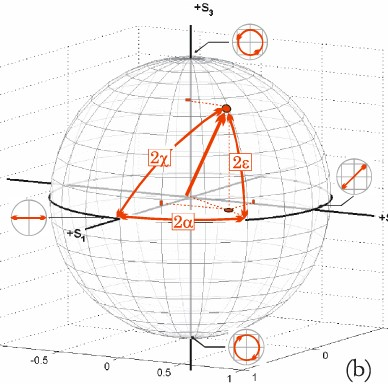
\includegraphics[width=0.7\linewidth]{./graphics/sphere}
\caption{longitude 2$\epsilon$ and latitude 2$\tau$}
\end{figure}
\begin{figure}[h]
\centering
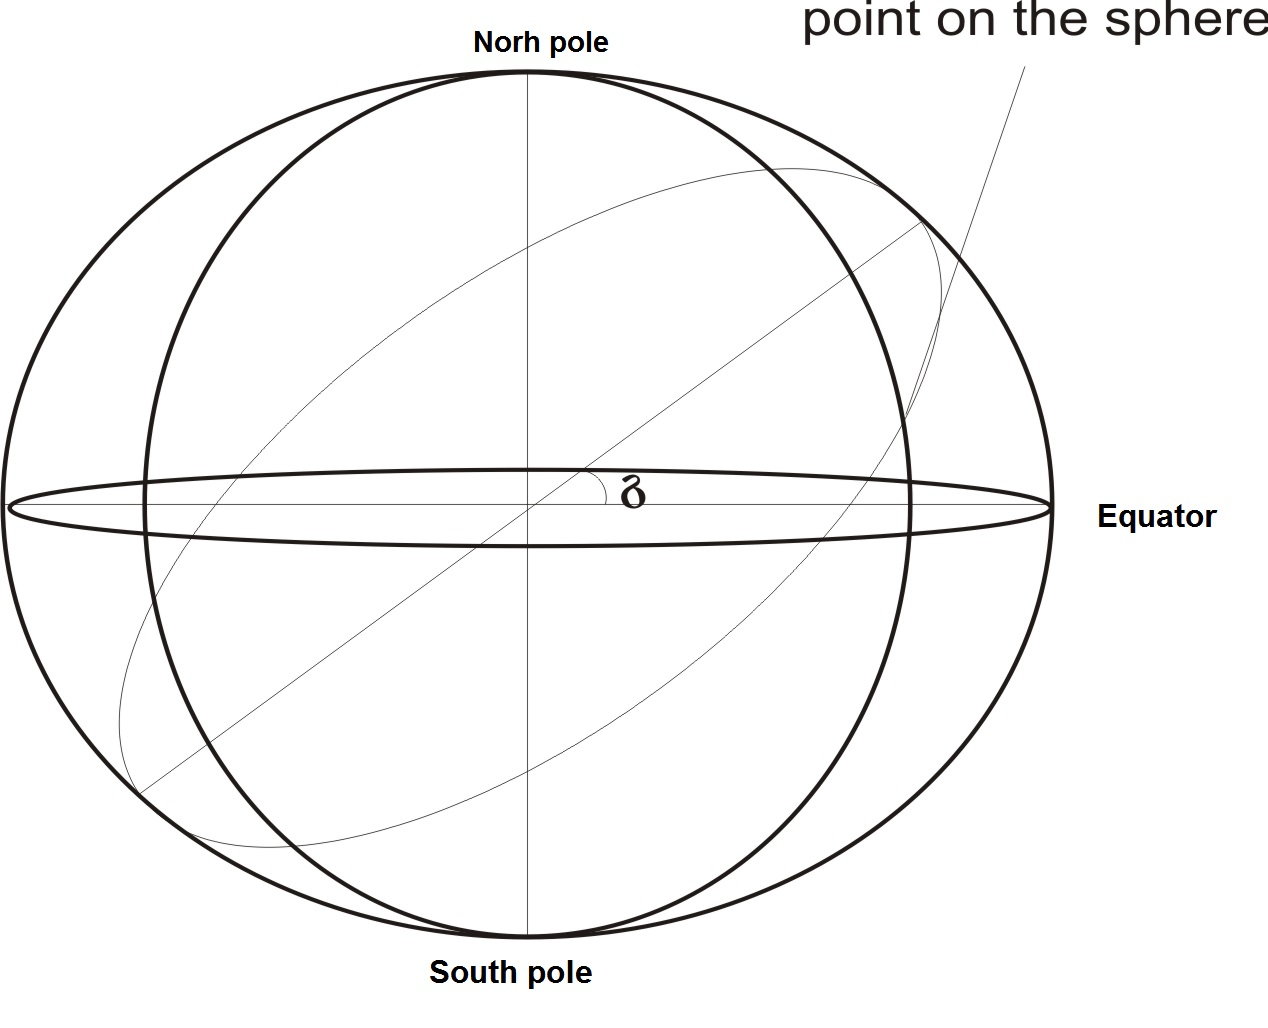
\includegraphics[height=5cm]{./graphics/SPHERE001}
\caption{Representation of $\delta$ on the Poincare Sphere}
\label{fig:sphere001}
\end{figure}

Essentially since the longitude varies from 0 to $360^{o}$, we will have a rotation around the sphere. This means that if we take the pair ($\epsilon$, $\tau$) for our representation where  2$\epsilon$ is the longitude and 2$\tau$ is the latitude, then all possible combinations of $\epsilon$ and $\tau$ are covered by the surface of the sphere.	Also, every point on the surface of the sphere has a unique combination of $\epsilon$ and $\tau$, which implies that every point on the sphere represents a unique state of polarization. All possible states of polarization are captured by the points on the sphere making this a very nice and compact representation of states of polarization.


\section{Conversion of wave parameters}
One could ask what are the special points on the sphere or what is the relationship between ($\gamma$, $\delta$) and ($\epsilon$, $\tau$).  

In getting the relationship between the electrical parameters and wave parameters, we have the horizontal plane which passes through the equator.
If we take a circle which passes through the reference point (centre of the sphere), the angle of the arc created by the circle, which is measured from the reference point to the point of the sphere is equal to 2$\gamma$.
If we have a plane passing through the reference point and the point on the sphere, the angle the plane makes with the horizontal plane of the sphere is equal to $\delta$.

Making use of spherical trigonometry\footnote{Spherical trigonometry is a branch of spherical geometry that deals with the relationship between trigonometric functions of the sides and angles of the spherical polygons e.g triangles, defined by several intersecting great circles on the sphere.}, we can find out the relationship between ($\epsilon$, $\tau$) and ($\gamma$, $\delta$), having marked all the angles in both the electrical domain and elliptical domain on the surface of the sphere. The relation is a conversion relation which enables the conversion of electrical parameters to elliptical parameters i.e from ($\gamma$, $\delta$) to ($\epsilon$, $\tau$) and also from the elliptical parameters to electrical parameters.

we have 
\begin{enumerate}[(i)]
\item Conversion from electrical parameters to elliptical parameters

$\tan(2\tau)$ = $\tan(2\gamma)$$\cos$$\delta$

$\sin(2\epsilon)$ = $\sin(2\gamma)$$\sin$$\delta$

If we are given electrical parameters, knowing the amplitude ratio of the two fields that will excite the electromagnetic wave and the phase difference between these two electric fields, we can find out the tilt angle and the axial ratio.
\item Conversion from elliptical parameters to electrical parameters.

$\cos(2\gamma)$ = $\cos(2\epsilon)\cos(2\tau)$

$\tan$$\delta$	= $\frac{\tan2\epsilon}{\sin2\tau}$
\end{enumerate}
When choosing the value of $\gamma$, $\delta$, $\epsilon$ or $\tau$ it should be kept in mind the range of values which satisfy each of them. By using this relation analytically one can convert the state of polarization in one domain to the other domain.

Going back to our Poincare sphere, as earlier, said the sphere represents all possible states of polarization. Let's examine some specific states of polarization. Going back to the parameters.
\begin{enumerate}[(i)]
\item Electrical parameters 

0$\leq$$\gamma$$\leq$$\pi$

$\dfrac{-\pi}{2}$$\leq$$\delta$$\leq$$\dfrac{\pi}{2}$
\item Ellipse parameters

$\dfrac{-\pi}{4}$$\leq$$\epsilon$$\leq$$\dfrac{\pi}{4}$

0$\leq$$\tau$$\leq$$\pi$
\end{enumerate}

\section{States of Polarization}
\subsection{Case 1: Linear Polarization}

\begin{figure}[h]
\centering
\includegraphics[height=5cm]{"./graphics/axial ratio"}
\caption{axial-ratio of an Ellipse}
\label{fig:axial-ratio}
\end{figure}

To get linear polarization;
\begin{enumerate}[(i)]
\item Axial ratio AR = $\infty$
\item $\dfrac{a}{b}$ = $\infty$, since b = 0,
\item $\epsilon$ = $\cot^{-1}$($\infty$) = $\tan^{-1}$($\dfrac{1}{\infty}$) = 0
\item $\tau = 0  $ to $  180^{o} $
\end{enumerate}
Looking at the reference point on the equator of the sphere, which is for measuring the longitude, the point corresponds to $\epsilon$ = 0 and $\tau$ = 0. This implies that, at the reference point when $\epsilon$ = 0, the axial ratio is infinite and $\tau$ = 0, the tilt angle is zero. This means that the point corresponds to a HORIZONTALLY LINEARLY POLARIZED WAVE.

If we move along the equator, changing the angle, the epsilon remains zero, which also makes the axial ratio remain infinite. However, the tilt angle goes on changing. At $\tau = 45^{o}$ and $2\tau = 90^{o}$, the line will be tilted at $45^{o}$ to the x-axis.

Moving round the sphere to the other side, at the opposite side to the reference point of the sphere, $\tau = 90^{o}$ and $2\tau = 180^{o}$, which means the tilt angle becomes $90^{o}$. The line becomes vertical. This is a VERTICALLY LINEARLY POLARIZED WAVE. 

So starting from the reference point, moving along the equator we have a horizontally polarized wave, while on the diagonally opposite point on the sphere we have a vertically polarized wave. If we continue moving along the equator towards the reference point, the line starts tilting and becomes horizontal at the reference point. This implies that all points along the equator represent all linear states of polarization.


\subsection{Case 2: Circular Polarization}
At the north pole of the sphere,
\begin{enumerate}[(i)]
\item 	$2\epsilon$ = $90^{o}$, 
\item	$\epsilon$ = $45^{o}$
\item	$\epsilon$ = $\cot^{-1}(\dfrac{a}{b})$
\item	$\dfrac{a}{b}$ = 1
\end{enumerate}
we see that the axial ratio is equal to one, which makes it a circle. For a circle, the tilt angle has lost its meaning and the major and minor axis are equal.

When axial ratio $(\dfrac{a}{b})$ = +1, this corresponds to a left-handed circular polarization.

In the same vane, at the south pole,
\begin{enumerate}[(i)]
\item	$2\epsilon$ = $-90^{o}$, 
\item $\epsilon$ = $-45^{o}$
\item $\epsilon$ = $\cot^{-1}(\dfrac{a}{b})$
\item $\dfrac{a}{b}$ = -1
\end{enumerate}	
This represents a right-handed circular polarization.

This implies that, any point which lies in the northern hemisphere, has a positive value i.e its axial ratio is positive, making that point which is in the northern hemisphere represent Left handed polarization.

We recall that if $E_{y}$ leads $E_{x}$, then we have a left-handed sense of rotation. If $E_{y}$ lags $E_{x}$, then the sense of rotation is right-handed. So any point in the northern hemisphere where $\delta$ $\neq$ 0 or $\delta$ $\neq$ $90^{o}$ represent left-handed elliptical polarization  (LHE), similarly any point in the southern hemisphere not at the equator or pole represents right-handed elliptical polarization (RHE).

So the Poincare sphere is a compact way of representing all the different states of polarization.

\section{Application of the Poincare sphere}
Let's say we have an electromagnetic wave coming with a vertical electric field, E (i.e vertically linearly polarized), say a piece of wire is placed vertically along the path of the incoming wave. From the basic knowledge of electromagnetism, voltage is induced in the wire ($\bar{E}$.$\bar{dl}$). If both wave and wire are parallel i.e both are vertical, $\bar{E}$.$\bar{dl}$ will be the induced voltage in the wire. If the wire is made horizontal and the angle between the wire and the wave is $90^{o}$, $\bar{E}$.$\bar{dl}$ = 0. As $ V = \bar{E}dl\cos\theta $, where $ \theta $ defines the relative angle between the field and wire.
\begin{figure}[h]
\centering
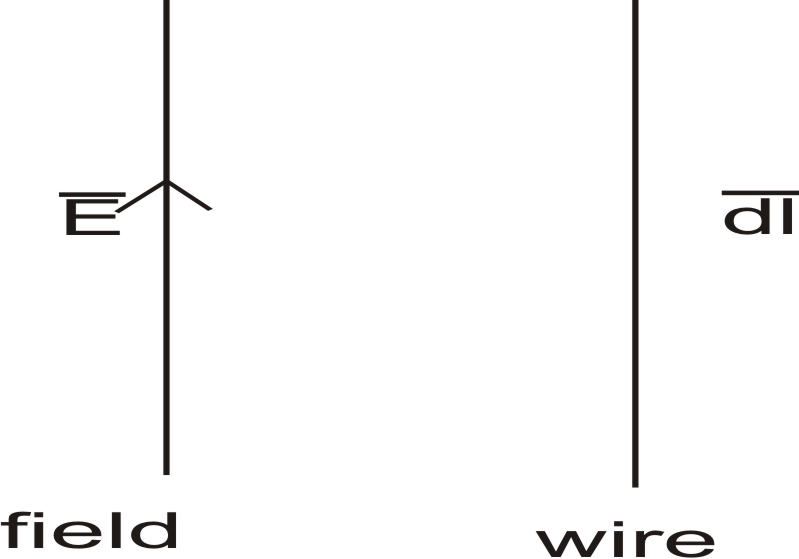
\includegraphics[width=.7\linewidth]{./graphics/interact}
\caption{Interaction between an Electric field and a wire}
\label{fig:interact}
\end{figure}

So although the field is existing and the wire is there, there is no induced voltage because of the relative angle between the field and the wire. This implies that the wire does not respond to the electric field.

This can be generalized to any system. If we have a system placed along the path of an electromagnetic wave, some voltage or current gets induced in the system and there is a power transfer from the wave to the system. Depending on the properties of the system and the properties of the electromagnetic wave there will be a certain amount of power exchange which will take place. Assuming the system was the wire, if the wire is vertical and the field is vertical, there is a maximum exchange of power but if the wire is horizontal and the field is vertical, there is zero exchange of power. If the wire were to be at an angle $\theta$ to the vertical axis, we will have an induced voltage which is smaller than $\bar{E}$.$\bar{dl}$ but greater than zero.

So we can say that for a system and an electromagnetic wave which is vertically polarized, if the system and the wave are both vertical there is maximum interaction and maximum power exchange but if the system is horizontal and the wave is vertical there is zero interaction and minimum power exchange.

This implies that the system has a state of polarization. This is defined as a state of polarization of that wave to which the system responds maximally.

Now we have two things, the state of polarization of the wave and the state of polarization Of the system. If both states of polarization matches, there is maximum power exchange between the wave and the system. If there is no exchange of power we say that the states of polarization are completely mismatched or the states of polarization are orthogonal to each other.

This concept can be applied to any arbitrary state of polarization, it is not confined to only linear polarization. We can take any state of polarization and find another state of polarization to which the system will respond maximally or to which it does not respond at all. So for every state of polarization, we can have its orthogonal state of polarization. 

What the Poincare sphere does essentially is that if the diagonally opposite point, on the surface sphere of a point, is taken, that point represents the orthogonal states of polarization. So One of the usefulness of the Poincare sphere is to find orthogonal states of polarization.

So point A on the surface of the sphere which is horizontally linearly polarized has a diagonally opposite point equal to $2\tau$ = $180^{o}$ which corresponds to vertical linear polarization. These are two states of orthogonal polarization. In the same manner, we can have a point which is left-handed circular (North pole) and diagonally opposite to this point is the right-handed circular polarization. These are two orthogonal states of polarization.

For the elliptical polarization, if a point of value of $\epsilon$ lies in the northern hemisphere, then the diagonally opposite point will lie in the southern hemisphere i.e the axial ratio will have the same value but an opposite sign. The $2\tau$ angle will increase by $2\tau = 180^{o}$ i.e the tilt angle will change by $90^{o}$.

So any two ellipses which have the same axial ratio, but the opposite sense of rotation and tilt angle shifted by $90^{o}$, will represent orthogonal states of polarization. The various orthogonal states of polarization discussed above are shown in fig\ref{fig:orthogonal states of polarization} below;

\begin{figure}[h]
	\centering
	\includegraphics[width=0.9\linewidth]{"./graphics/orthogonal_states"}
	\caption{Orthogonal states of polarization}
	\label{fig:orthogonal states of polarization}
\end{figure}

\section{Generating elliptical states of polarization from an orthogonal pair}
First, let's recall that linear and circular polarization are special cases of elliptical polarization. 

Now let's go back to the electric field vector, which is a combination of $E_{x}$( which is a horizontally polarized wave) and $E_{y}$(which is a vertically polarized wave). Now let's see why $E_{x}$ and $E_{y}$ could generate any arbitrary ellipse because we are talking about two orthogonal states of polarization. i.e by combining the two, $E_{x}$ and $E_{y}$ we could generate any arbitrary elliptic state of polarization.

Instead of using linear polarization, we shall be using circular polarization to generate our arbitrary ellipse. Two circular orthogonal polarization, Left-handed circular(LHC) and Right-handed circular(RHC) pair. From the combination of these two, we can generate any arbitrary state of polarization. 

We have two states of orthogonal polarization, two waves of the same amplitude but rotating in opposite directions. In a superposition of the two vectors in space, the resulting electric field will simply move in the horizontal plane giving us a linear polarization.

\begin{enumerate}[(i)]
\item At time t = 0, both arrows point in the same direction, adding up to give the point 0 on the line below.
\item At a time $ t_{1} $, LHC will move to point 1 (counterclockwise rotation) and RHC wave move to point 1 (clockwise rotation), adding up vectorially to get point 1 on the line below.
\item At a time $ t_{2} $, LHC will move to point 2 (counterclockwise rotation) and RHC wave move to point 2 (clockwise rotation), adding up vectorially to get point 2 on the line below.
\item At a time $ t_{3} $, LHC will move to point 5 (counterclockwise rotation) and RHC wave move to point 5 (clockwise rotation), adding up vectorially, they will cancel out as they are equal and opposite in direction.
\item At a time $ t_{4} $, LHC will move to point 4 (counterclockwise rotation) and RHC wave move to point 4 (clockwise rotation), adding up vectorially to get point 4 on the line.
\end{enumerate}

\begin{figure}[h]
	\centering
	\includegraphics[width=1\linewidth]{"./graphics/generatingEP"}
	\caption{Generating elliptic states of polarization from an orthogonal pair}
	\label{fig:linear-polarized}
\end{figure}

In the end, we have a linearly polarized wave by adding two orthogonal circular polarized waves.

The circular polarization is taken as the primary polarization. Since the two circular polarized waves constitute an orthogonal set, we can generate any arbitrary polarization from them. If we take different values of amplitude and phase i.e manipulate the circle parameters, we can get different states of polarization from the primary circularly polarized wave. This implies that by using two states of orthogonally polarized waves, any arbitrary state of polarization can be generated.


\section{Application of orthogonal state of polarization in communication system}	
Generating any arbitrary states of polarization can be done using any two states of orthogonal systems. Orthogonal states of polarization are quite useful in practice. For instance, if we have two orthogonal systems, there is no interaction between the two systems, and there is a possibility of sending two signals at the same time in space at the same frequency by using two orthogonal states of polarization for two signals. Even if they are mixed in space at the receiver, the two signals having orthogonal states of polarization can be separated. By using polarization, we can increase the capacity by sending information by a factor of 2. This is because we can put independent information in the two states of polarization and since we have a mechanism for separating the states of polarization by choosing a system with a particular polarization, the information can always be separated.	
\begin{figure}[h]
\centering
\includegraphics[height=5cm]{"./graphics/orthogonal polarized wave"}
\caption{orthogonal States of polarized wave}
\label{fig:orthogonal-polarized-wave}
\end{figure}


\section{Efficiency of power transfer}
The Poincare sphere also gives us information about the efficiency of power transfer between a system and a wave with their respective states of polarization. If the states of polarization of the wave and the system are represented by M and M' respectively on the Poincare sphere as shown below;

\begin{figure}
	\centering
	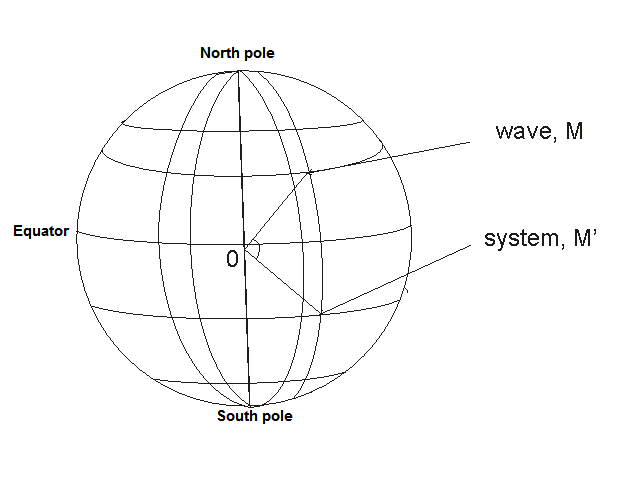
\includegraphics[width=1\linewidth]{./graphics/power}
	\caption{Determination of efficiency of power transfer}
	\label{fig:power}
\end{figure}

The angle which points $M$ and $M^'$ subtends at the centre of the Poincare sphere can be used to calculate the efficiency of power exchange.
The angle is at MOM' if the centre of the sphere is at O. The efficiency of power exchange is given by,

\[\eta = \cos^2 {\frac{ \angle  MOM' }{2}}  \]

The Poincare sphere can therefore also be used to find the efficiency of power transfer between the wave and the system. Examining some specific cases of power transfer between the wave and the system, we see that for a linearly polarized system, M' is on the horizontal equator plane, and for a circularly polarized wave, M is at the pole, thus $\angle MOM' = 90^o$.
\[ \eta= \cos ^2(\frac{90^o}{2}) =\cos ^2(45^o) =(\frac{1}{\sqrt{2}})^2  = \frac{1}{2}\]

So circularly polarized waves and linearly polarized systems or vice versa have an efficiency of power exchange $ \eta=  50\% $. So even if the state of polarization of the system changes in rotation on the equator i.e from horizontal to vertical linearly polarized as long as the other wave it is interacting with is circularly polarized, the efficiency will remain 50\%.

So in practice, if we have a situation where the field vector is varying as a function of time but remains linear and we use a receiving system which is circularly polarized, we will always have a constant output since efficiency is 50\%. However, when we have a linearly polarized system and a linearly polarized wave, if the angle between them changes, the efficiency will also keep changing because the dot product between $ \bar {E} $ and $ \bar{dl} $ will keep changing. This is the situation we have in Satellite communication. The electric field experiences constant rotation as a result of the ionosphere. This phenomenon is referred to as Faraday's rotation\footnote{This is a magneto-optical phenomenon i.e interaction between light and magnetic field in a medium. It causes a rotation of the plane of the magnetic field in the direction of propagation.}. If the receiving antenna of that electric field is linearly polarized, the output keeps changing as a function of time as the electric field and receiving system keep changing angle with respect to each other. Assuming the receiving antenna is circularly polarized and the wave coming is linearly polarized, even if the linearly polarized wave changes its direction, the efficiency will always be 50\% and we get a guaranteed output i.e we do not see any fluctuation in the output. Using the concept of polarization, many innovative things can be done in communication systems and of course there are many factors which essentially decide what the polarization of the receiving system should be.

Hence, the polarization of an electromagnetic wave plays a very important role in designing communication systems. Before one goes into the design of communication systems, this aspect of the electromagnetic wave must be understood thoroughly. Polarization of electromagnetic waves also finds applications in lasers, radar, wireless and optical fibre telecommunications, and display technologies e.g LCD.

\section{Summary}
\begin{enumerate}[(i)]
\item Wave polarization is the behaviour of the electric field as a function of time at a given point in space. We have three types of polarization; linear, circular and elliptical polarization.
\item States of polarization can be described by Electrical and elliptical(wave) parameters. \\
\\
\begin{tabular}{|l|m{4.5cm}|}
	\hline 
	\textit{Representation} &\textit{Parameters} \\ \hline % row one 
	Electrical Parameters &  $ (\frac{E_{2}}{E_{1}}, \delta)\hspace{0.15cm}  \text{and } (\gamma, \delta)\hspace{0.15cm} \text{where, } \gamma = \arctan(\frac{E_{2}}{E_{1}}) $\\  \hline     % row two 
	Wave Parameters & $ (\pm AR, \tau)\hspace{0.15cm}  \text{and } (\epsilon, \tau)\hspace{0.15cm} \text{where, } \epsilon = cot^{-1}(\pm AR) $ \\ \hline % row three
\end{tabular} \\
\\
\item These parameters have a range of angles. For Electrical parameters; $ 0 \leq \gamma \leq \pi $ and $ -\frac{\pi}{2} \leq \delta \leq \frac{\pi}{2}$. For Ellipse(wave) parameters; $ -\frac{\pi}{4} \leq \epsilon \leq \frac{\pi}{4}$ and $ 0 \leq \tau \leq \pi $.
\item These parameters can be used to construct a sphere called The Poincare sphere. This Poincare sphere has points capable of representing all possible states of polarization.
\item  Orthogonal pair consists of two systems which are capable of cancelling each other when they interact. Orthogonal pairs of polarization are capable of generating any arbitrary state of polarization. The knowledge of orthogonal pairs finds practical relevance in increasing the volume of information transmitted in transmission systems. 
\item The Poincare sphere can be used to find a corresponding orthogonal point on its surface from a given reference point. The Poincare sphere also gives information about the power exchange between a system and a field represented on its surface.
\item The knowledge of states of polarization is very important in the design of communication systems to maximize the efficiency of these systems. 
\item  Polarization of electromagnetic waves finds applications in lasers, radar, wireless and optical fibre telecommunications, and display technologies e.g LCD.
\end{enumerate}